\documentclass[10pt, tikz, border=2mm]{standalone}
\usetikzlibrary{arrows.meta, positioning}

\begin{document}
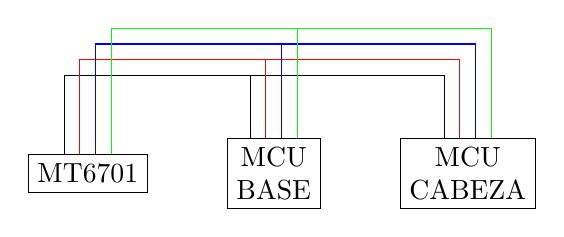
\begin{tikzpicture}[every node/.style={align=center}]
    \node[rectangle, draw=black] (sensor) {MT6701};
    \node[rectangle, draw=black, right=1cm of sensor] (mcu) {MCU\\ BASE};
    \node[rectangle, draw=black, right=1cm of mcu] (mcu2) {MCU\\ CABEZA};

    \draw ([xshift=-3mm]sensor.north) -- ++(0,1) coordinate(ground)
    -| ([xshift=-3mm]mcu.north);
    \draw (ground) -| ([xshift=-3mm]mcu2.north);
    \draw[red] ([xshift=-1mm]sensor.north) -- ++(0,1.2) coordinate(ground)
    -| ([xshift=-1mm]mcu.north);
    \draw [red] (ground) -| ([xshift=-1mm]mcu2.north);
    \draw [blue] ([xshift=1mm]sensor.north) -- ++(0,1.4) coordinate(ground)
    -| ([xshift=1mm]mcu.north);
    \draw [blue] (ground) -| ([xshift=1mm]mcu2.north);
    \draw [green] ([xshift=3mm]sensor.north) -- ++(0,1.6) coordinate(ground)
    -| ([xshift=3mm]mcu.north);
    \draw [green] (ground) -| ([xshift=3mm]mcu2.north);
\end{tikzpicture}
\end{document}
